\documentclass[presentation]{beamer}   % to compile the presentation
%\documentclass[handout]{beamer}        % to compile 2x2 handouts
\usepackage[ansinew]{inputenc}
\usepackage[T1]{fontenc}
\usepackage{lmodern,textcomp}
\usepackage{breakurl}
\usepackage{graphicx}
\usetheme{Singapore}
\usepackage[formats]{listings}
\lstdefineformat{C}{% 
	\{=\newline\string\newline\indent,% 
	\}=[;]\newline\noindent\string\newline,% 
	\};=\newline\noindent\string\newline,% 
	;=[\ ]\string\space}
\lstset{language=C}

%\usepackage{/usr/lib64/R/share/texmf/Sweave}
%\usepackage{/Library/Frameworks/R.framework/Resources/share/texmf/Sweave}
\setbeamercovered{transparent}

\begin{document}
% The DTU and MIC logos
\pgfdeclareimage[height=2cm]{dtulogo}{dtu_logo}
%\pgfdeclareimage[width=0.8\framesep]{miclogo}{mic_logo}

\author{Sigmar Stef\`{a}nson and Francesco Favero}
\title{Stabilization Matrix Method}
\date{29 Oct. 2010}
\institute[ CBS - Algorithms in Bioinformatics]{DTU}
\titlegraphic{\pgfuseimage{dtulogo}} % Graphics for title slide
%\logo{\pgfuseimage{miclogo}} % The left logo



\begin{frame}
  \maketitle
\end{frame}

%\begin{frame}
%  \frametitle{Outline}
%  \tableofcontents[currentsection]
%\end{frame}

\section{Code Change}
\begin{frame}
  \frametitle{Code Change}
  \begin{block}\centering
  	We used brute-force method to evaluate the optimal lambda. To be able to run the smm algorithm as efficiently as possible we made some minor changes. Some of these changes are probably made by the compiler optimization.
  \end{block}
   \pause
  \begin{block}\centering
  	Another change we made was the ability to evaluate model efficiency on training and testing data for each cycle side by side. The test data file is then an extra parameter to the program.
  \end{block}
\end{frame}

\begin{frame}[fragile,plain]
Our update\_weight implementation, optimization mainly involving join of parameters and removal of memory allocation.
 \begin{lstlisting}[basicstyle=\scriptsize,format=C]

inline void update_weight(float *w,float *inp,float d_o,int n) {
	int j;
	float p_etad_o = p_eta * d_o;
	for ( j=0; j<n; j++ ) {w[j] -= p_etad_o * inp[j] + p_eta2lambda * w[j];
	}
}
  \end{lstlisting}
\end{frame}

\begin{frame}[fragile,plain]
\frametitle{Training vs testing Pearson correlation coefficient}
We added the ability to be able to watch testing PCC and MSE for each step in the training (in addition to the training values). The purpose of this was to be able to investigate over-fitting.
		\begin{figure}
		\centering
			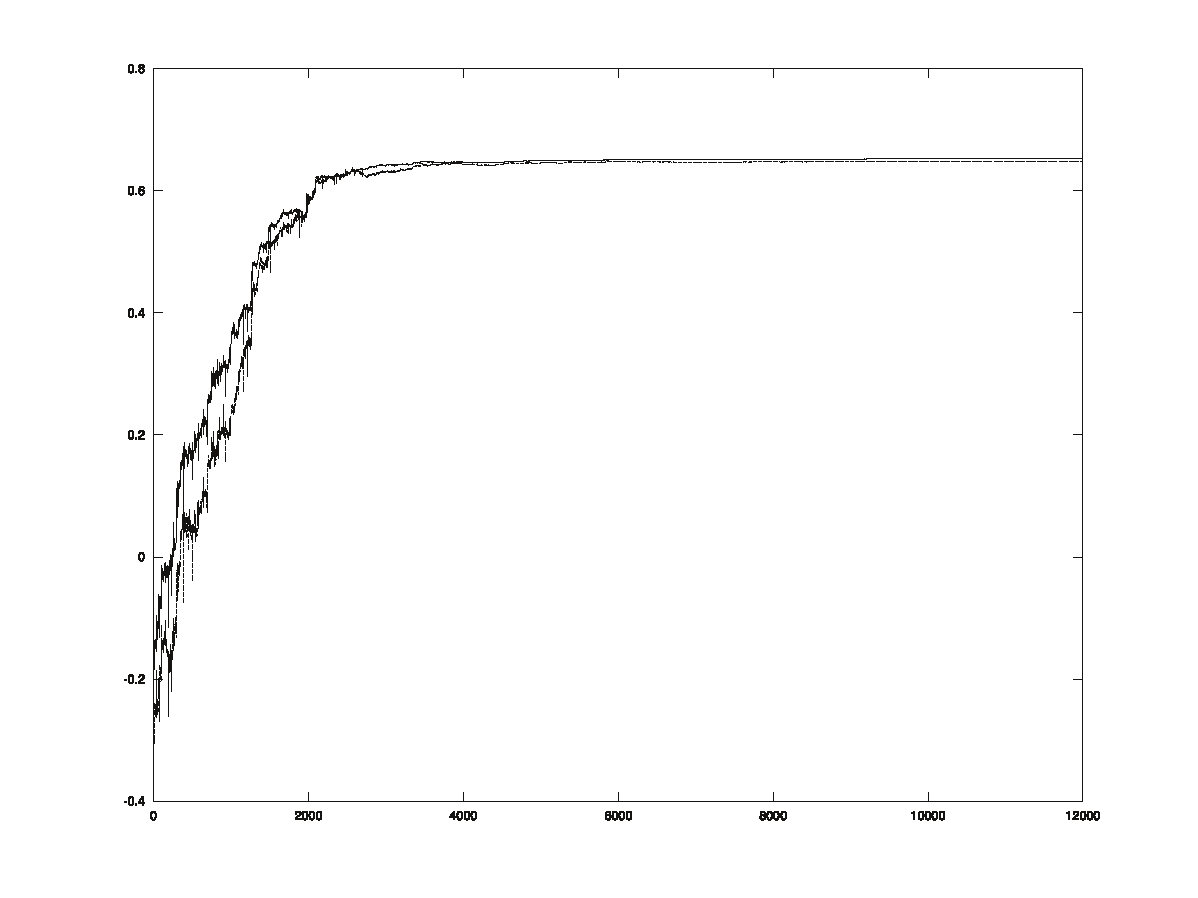
\includegraphics[width=90mm,height=60mm]{fig/pcc2.pdf}
			\caption{Training vs testing PCC}
		\end{figure}
\end{frame}

\begin{frame}[fragile,plain]
\frametitle{Difference in error values for Monto Carlo and Gradient Descent implementations for 12000 and 500 iterations respectively}
\begin{columns}[t] % Align the columns at the top
    \column{0.4\textwidth}
		\begin{figure}
		\centering
			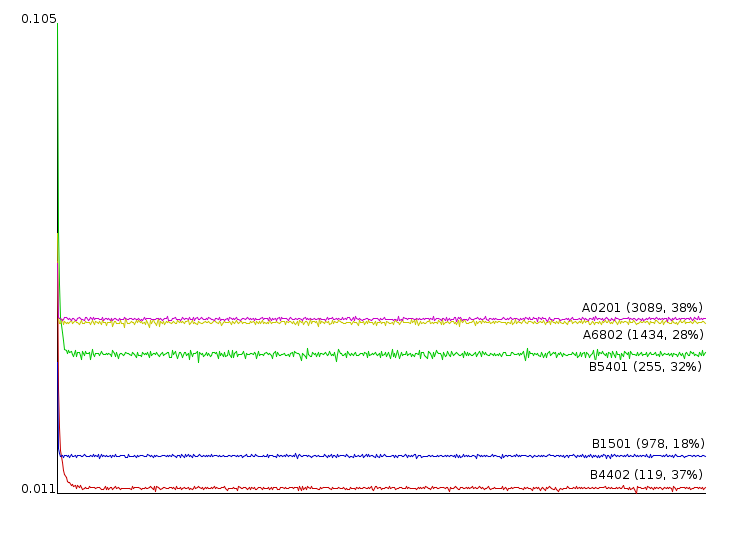
\includegraphics[width=40mm,height=40mm]{fig/smm_error.png}
			\caption{Gradient decent}
		\end{figure}
  	\column{0.6\textwidth}
		\begin{figure}
			\centering
			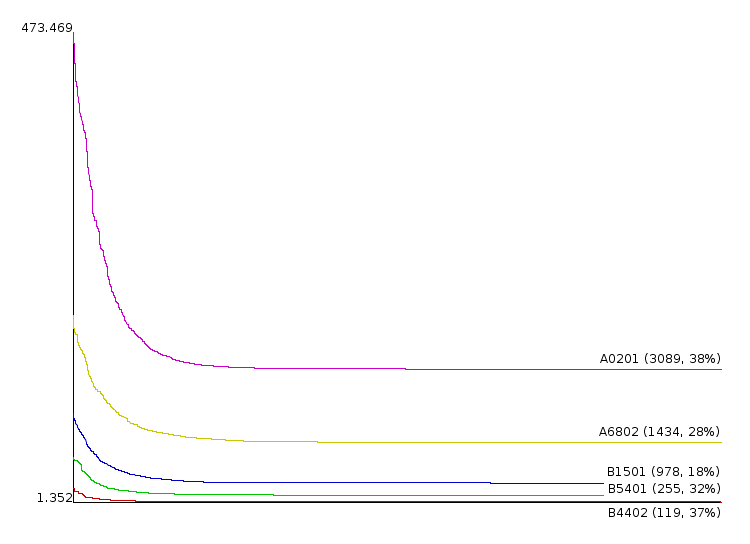
\includegraphics[width=40mm,height=40mm]{fig/smm_mc_error.png}
			\caption{Monte Carlo}
		\end{figure}
  \end{columns}
\end{frame}

\section{Correlation and $\lambda$}
\begin{frame}
  \frametitle{Size depending Pearson correlation coefficent}
  \begin{columns}[t] % Align the columns at the top
    \column{0.4\textwidth}
		\begin{figure}
		\centering
			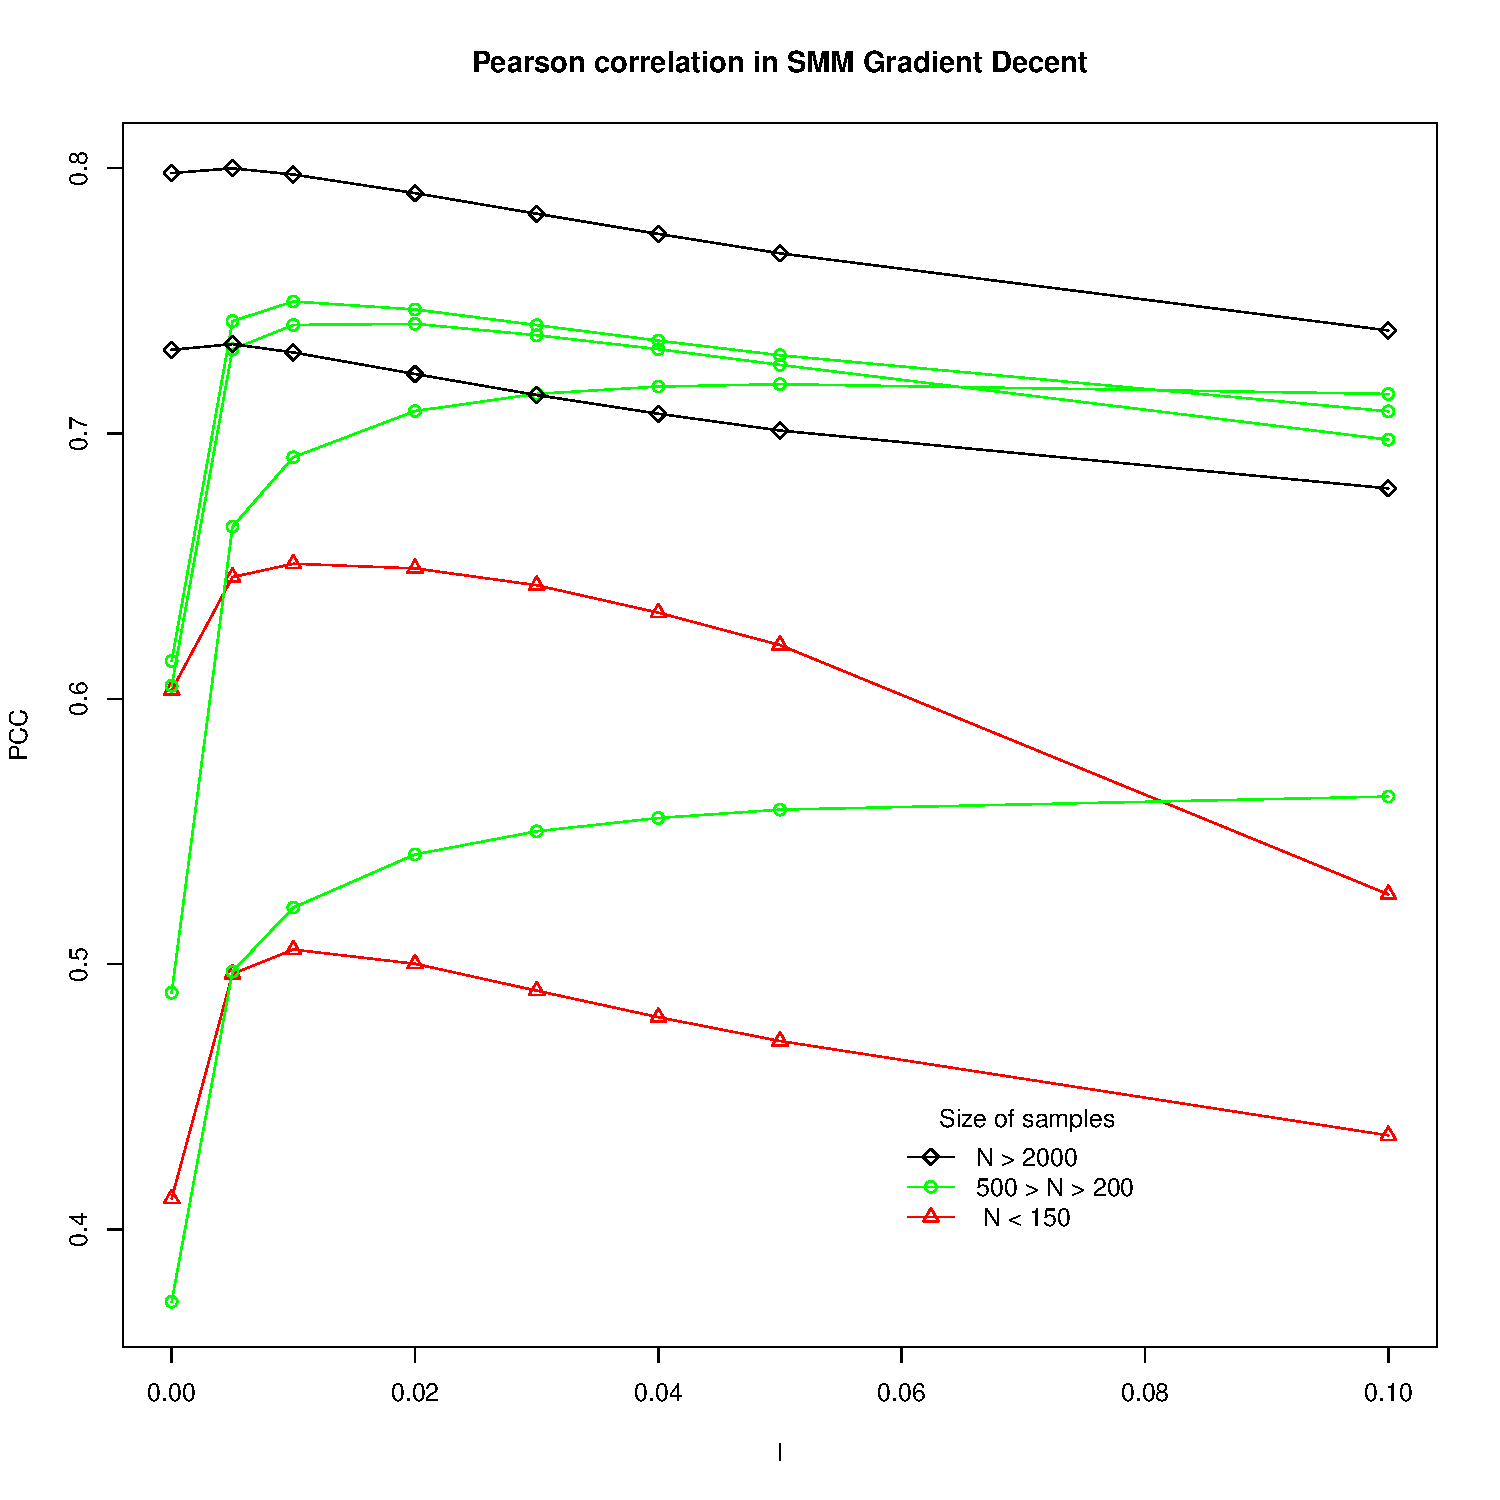
\includegraphics[width=40mm,height=40mm]{fig/smm_l005_ppc_size.pdf}
			\caption{Gradient decent}
		\end{figure}
  	\column{0.6\textwidth}
		\begin{figure}
			\centering
			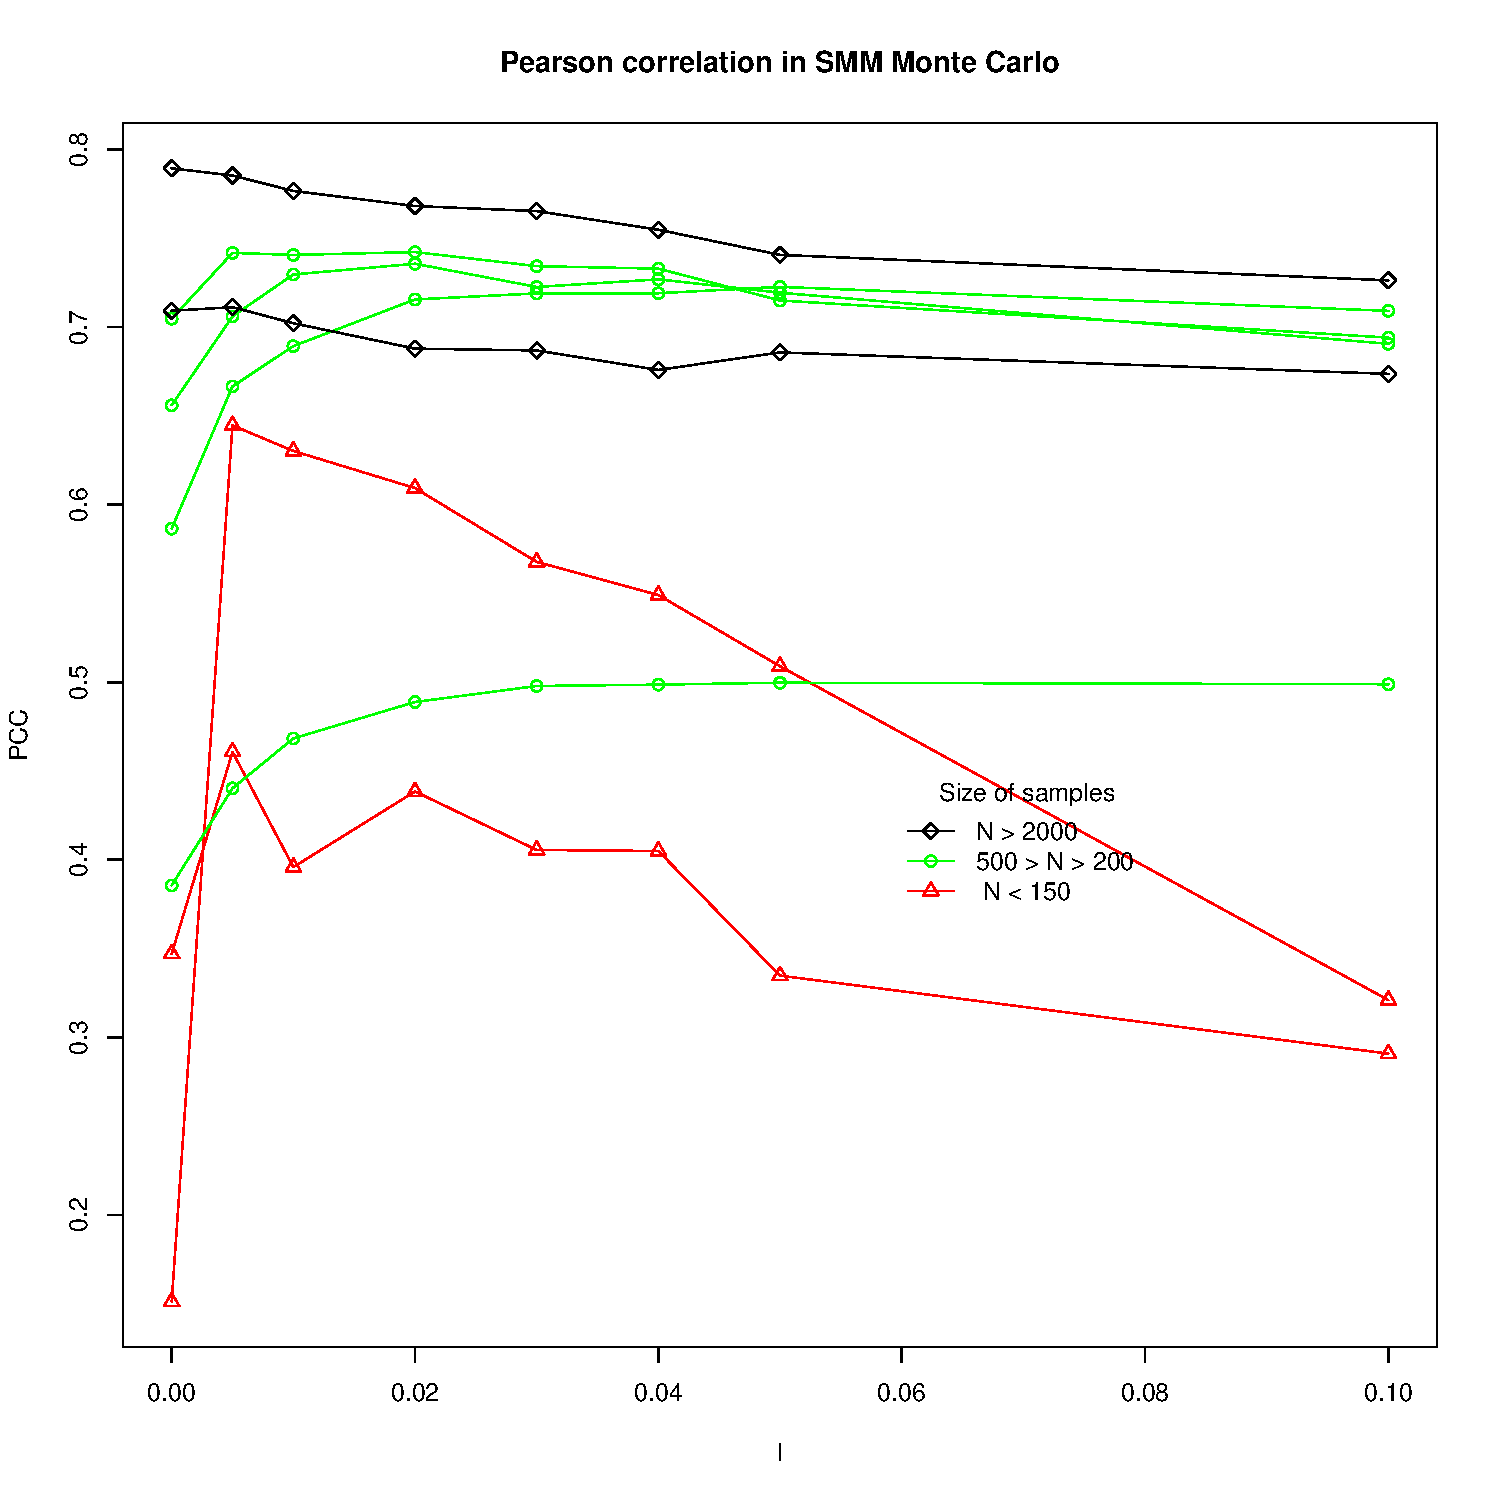
\includegraphics[width=40mm,height=40mm]{fig/smm_mc_l005_ppc_size.pdf}
			\caption{Monte Carlo}
		\end{figure}
  \end{columns}
\end{frame}

\begin{frame}[plain]
  \frametitle{Choice of best $\lambda$ value}
	\begin{figure}
	\centering
		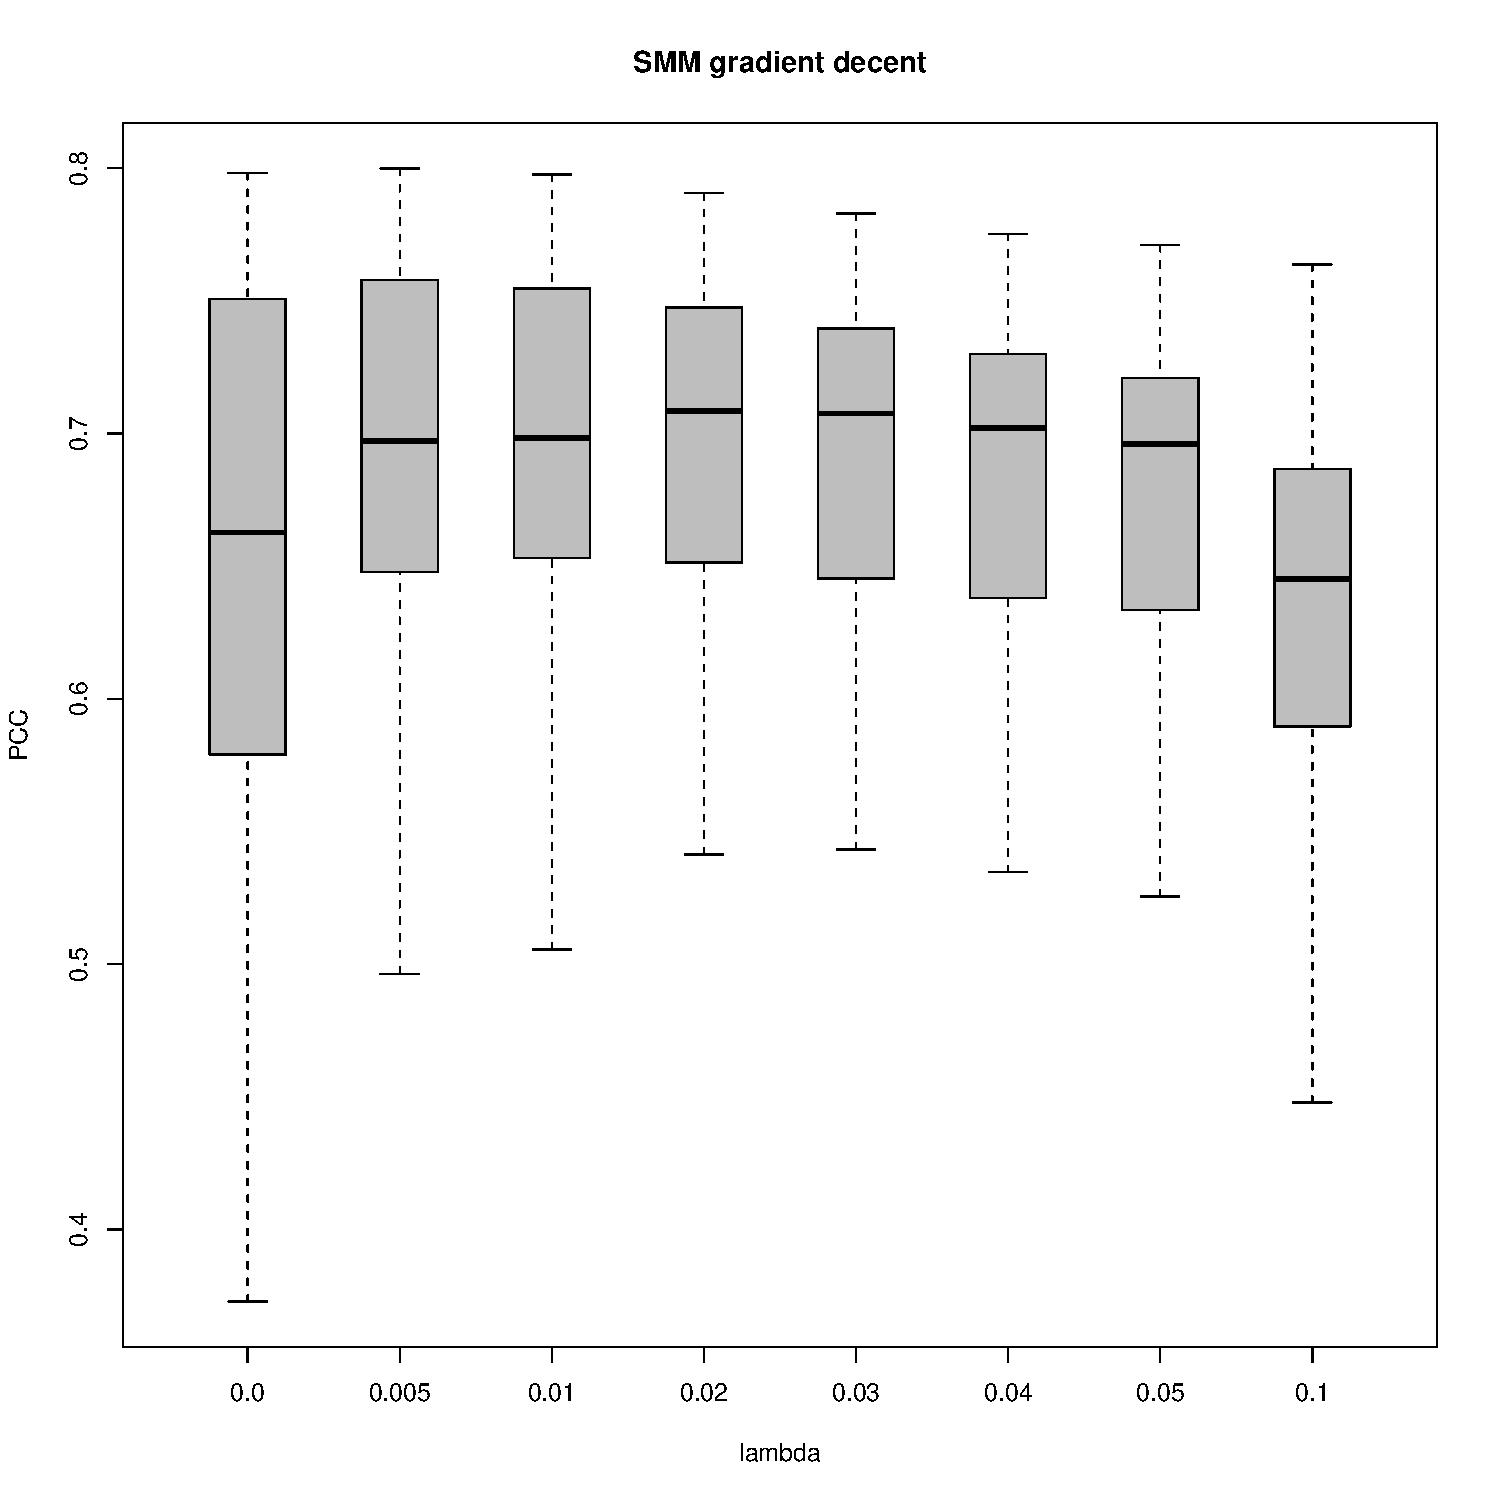
\includegraphics[width=70mm,height=70mm]{fig/choice_lambda.pdf}
		\caption{Gradient decent}
	\end{figure}
\end{frame}

\begin{frame}[plain]
  \frametitle{Choice of best $\lambda$ value}
	\begin{figure}
		\centering
		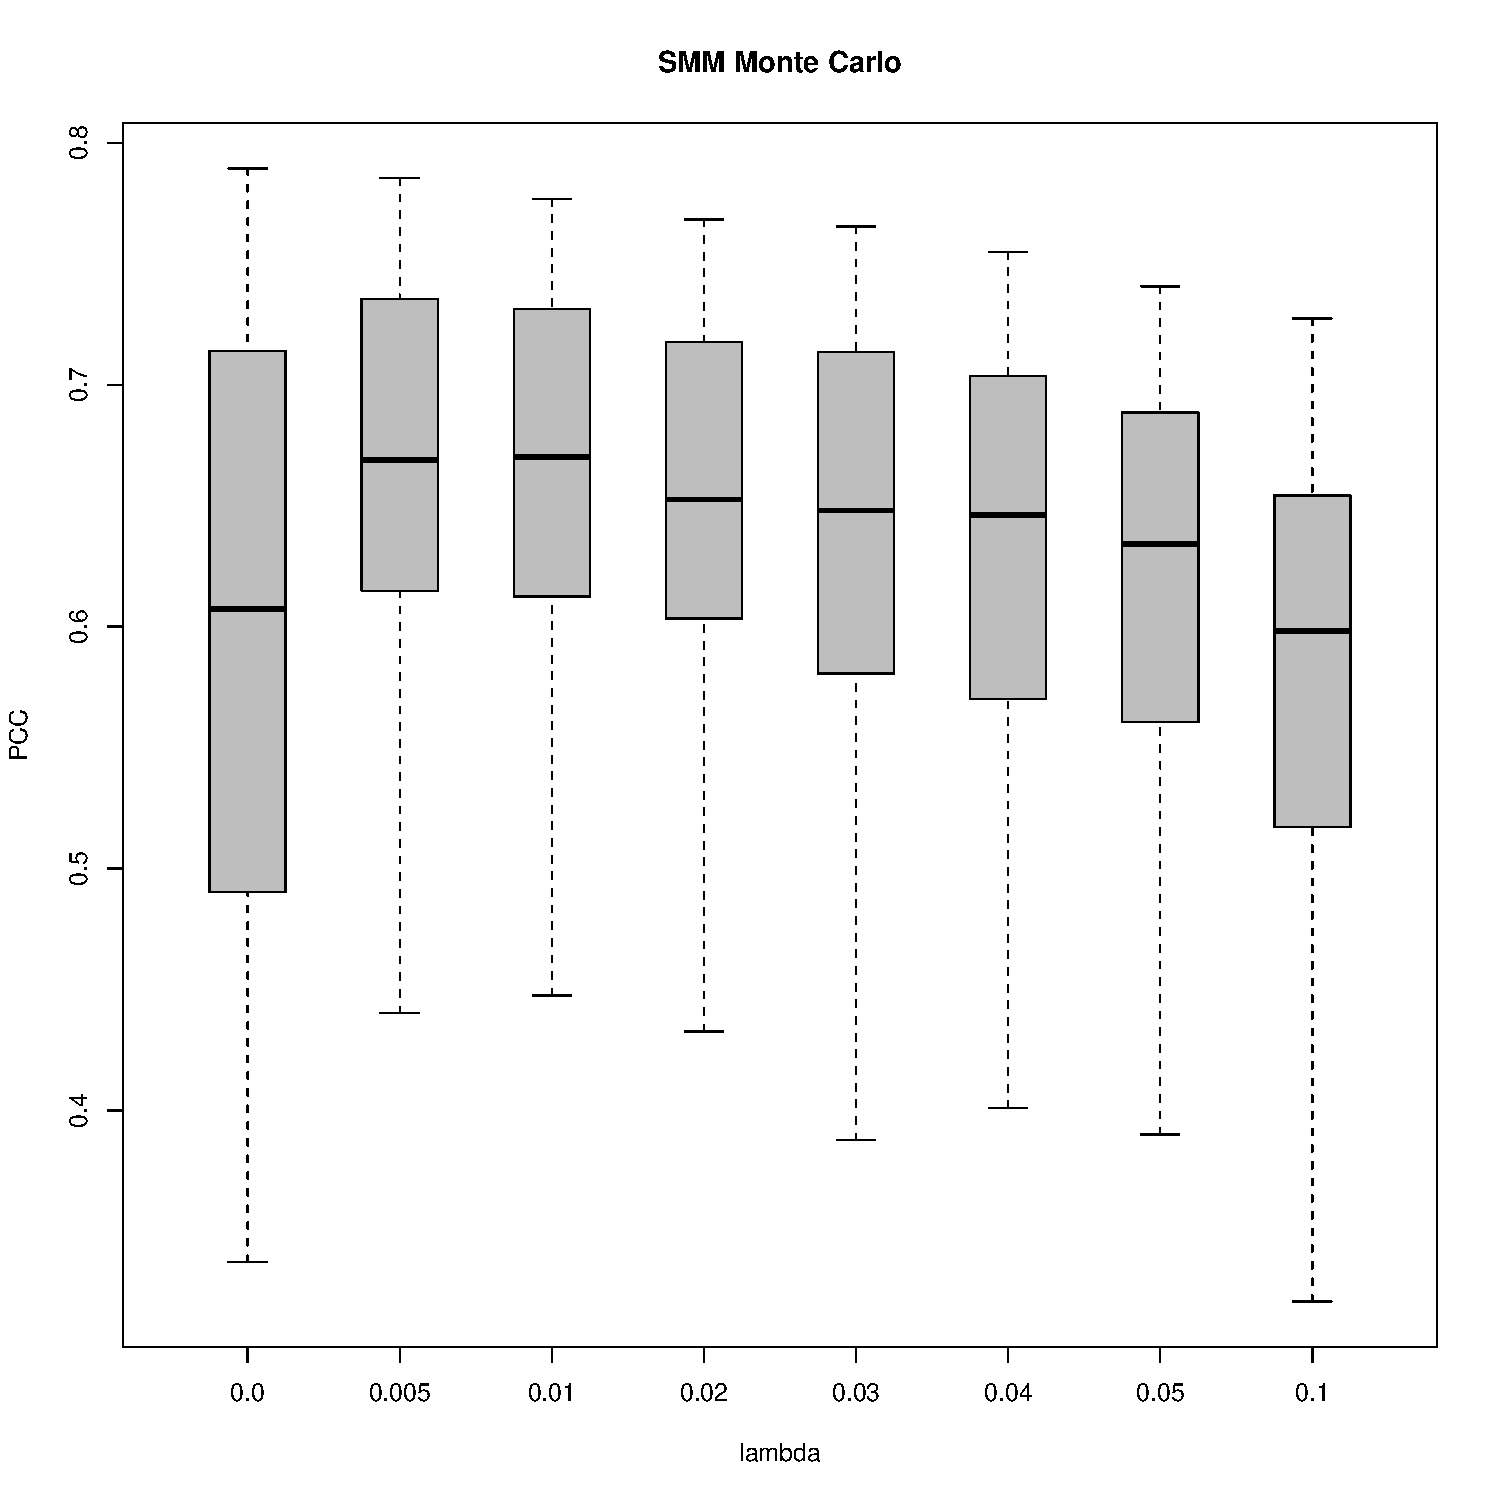
\includegraphics[width=70mm,height=70mm]{fig/choice_lambda_mc.pdf}
		\caption{Monte Carlo}
	\end{figure}
\end{frame}

\section{Conclusion}
\begin{frame}
\begin{itemize}
\item 1 \pause
\item 2 \pause
\item 3
\end{itemize}
\end{frame}
\begin{frame}[plain]
	\begin{figure}
	\centering
	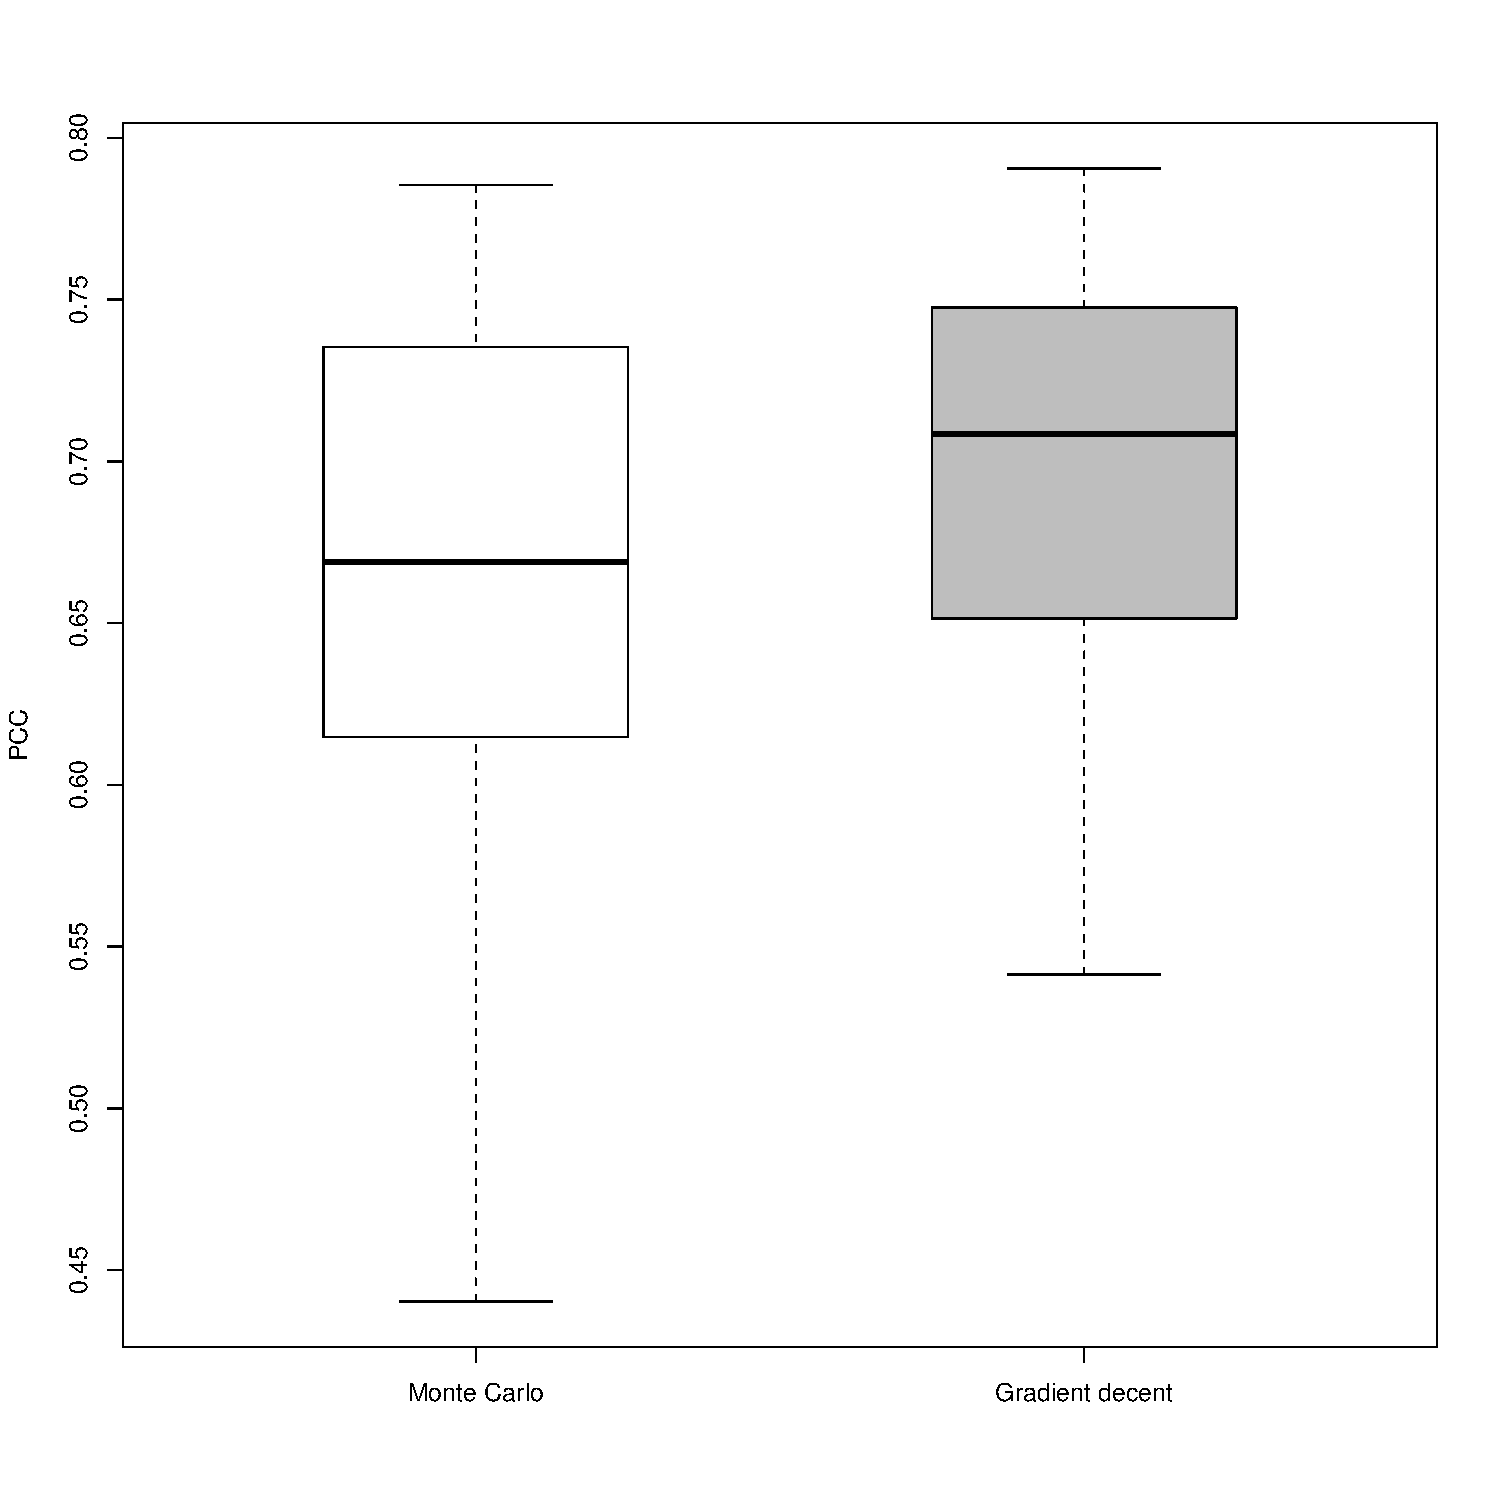
\includegraphics[width=80mm,height=80mm]{fig/boxplot.pdf}
	\caption{blablabla}
	\end{figure}
\end{frame}

\end{document} 
